\documentclass[10pt,journal,twoside]{IEEEtran}
\vfuzz=2pt
\IEEEoverridecommandlockouts
\usepackage{amsmath,amssymb,amsfonts,amsthm,mathtools,bm}
\usepackage{booktabs,array,graphicx,cite,url,float,stfloats,microtype,xcolor}
\definecolor{IEEElinkblue}{HTML}{00629B}
\usepackage[colorlinks=true,linkcolor=IEEElinkblue,citecolor=IEEElinkblue,urlcolor=IEEElinkblue,breaklinks=true]{hyperref}
\newtheorem{proposition}{Proposition}
\newtheorem{definition}{Definition}
\newtheorem{assumption}{Assumption}
\newfloat{algorithm}{tbp}{loa}
\floatname{algorithm}{Algorithm}
\newcommand{\cV}{\mathcal{V}}
\newcommand{\cZ}{\mathcal{Z}}
\newcommand{\cU}{\mathcal{U}}
\newcommand{\cA}{\mathcal{A}}
\newcommand{\R}{\mathbb{R}}
\newcommand{\E}{\mathbb{E}}
\newcommand{\norm}[1]{\left\lVert #1\right\rVert}
\newcommand{\ind}{\mathbf{1}}
\newcommand{\alghead}[1]{\multicolumn{2}{@{}p{0.94\columnwidth}@{}}{\textbf{#1}}\\}
\newcommand{\DatasetRows}{201,912}
\newcommand{\TrainingRows}{109,539}
\newcommand{\TestRows}{92,373}
\newcommand{\StableNrmse}{0.685}
\newcommand{\StableAgreement}{91.33\%}
\newcommand{\NrmseGainBest}{4.5\%}
\newcommand{\AgreementGainBest}{0.96 percentage points}
\newcommand{\StableCoverage}{94.35\%}
\newcommand{\StableAcceptance}{53.53\%}
\newcommand{\StableSelectiveError}{0.233\%}
\newcommand{\DriftDetection}{90.6\%}
\newcommand{\DriftDelay}{8.96~s}
\newcommand{\DriftFalseAlarm}{9.4\%}
\newcommand{\DriftSelectiveError}{5.39\%}
\newcommand{\NoDriftSelectiveError}{51.2\%}
\newcommand{\DriftErrorReduction}{89.5\%}
\newcommand{\BridgeLatency}{22.1~$\mu$s/sample}
\newcommand{\BridgeModelSize}{1.44~MiB}
\newcommand{\CertificateBytes}{48~B}
\newcommand{\HundredUeCertificateRate}{0.384~Mbit/s}

\setlength{\textfloatsep}{7pt plus 1pt minus 2pt}
\setlength{\dbltextfloatsep}{7pt plus 1pt minus 2pt}
\setlength{\floatsep}{5pt plus 1pt minus 2pt}
\setlength{\intextsep}{5pt plus 1pt minus 2pt}
\setlength{\abovedisplayskip}{4pt plus 1pt minus 1pt}
\setlength{\belowdisplayskip}{4pt plus 1pt minus 1pt}
\setlength{\abovecaptionskip}{3pt}
\setlength{\belowcaptionskip}{0pt}

\title{KPM-Bridge: An Uncertainty-Aware Cross-Implementation Telemetry Fabric for Portable AI xApps in Open 6G RAN}

\author{Yassir~AL-Karawi and Hamed~Al-Raweshidy%
\thanks{Y. AL-Karawi is with the College of Engineering, University of Diyala, Baqubah, Iraq (e-mail: yassirameen22@gmail.com).}%
\thanks{H. Al-Raweshidy is with the Wireless Networks and Communications Centre, College of Engineering, Design and Physical Sciences, Brunel University of London, Uxbridge UB8 3PH, U.K. (corresponding author; e-mail: hamed.al-raweshidy@brunel.ac.uk).}%
}

\begin{document}
\bstctlcite{IEEEexample:BSTcontrol}
\maketitle

\begin{abstract}
Two Open Radio Access Network (O-RAN) implementations may emit valid E2 Service Model for Key Performance Measurement (E2SM-KPM) reports while assigning different meanings to the same artificial-intelligence (AI) xApp input. Units, entity scope, windows, clocks, counter resets, missingness, and filtering can all differ. KPM-Bridge treats this as a typed translation problem: it compiles source contracts, aligns event-time observations, learns an anchor-assisted map $M_v:y_{v,\le t}\mapsto\hat z_t$, and attaches a 48-byte evidence certificate. Split-conformal sets cover both $z_t\in\R^d$ and a registered xApp functional $\ell(z_t)$. On \DatasetRows\ public ColO-RAN samples with experiment-level separation, seven baselines, controlled profiles, and ablations, KPM-Bridge obtains \StableNrmse\ normalized root-mean-square error and \StableAgreement\ decision agreement across three stationary profiles; reductions relative to the strongest respective baselines are \NrmseGainBest\ and \AgreementGainBest. At nominal miscoverage $\alpha=.05$, joint coverage is \StableCoverage, while accepted actions have \StableSelectiveError\ disagreement at \StableAcceptance\ acceptance. Under severe drift, the monitor detects \DriftDetection\ of shifted traces with \DriftDelay\ median delay. Fail-closed invalidation changes post-shift disagreement exposure from \NoDriftExposure\ to \DriftExposure\ by reducing acceptance to 5.99\%; conditional disagreement remains \DriftSelectiveError. These profiles are controlled stressors, not commercial-vendor measurements.
\end{abstract}

\begin{IEEEkeywords}
6G, Open RAN, E2SM-KPM, xApp portability, conformal prediction.
\end{IEEEkeywords}

\section{Introduction}
\IEEEPARstart{O}{pen} Radio Access Network (O-RAN) architectures disaggregate the radio access network (RAN), expose standardized interfaces, and host programmable control applications in a near-real-time RAN Intelligent Controller (Near-RT RIC) \cite{polese2023understanding,alam2026survey,garcia2021oran}. This arrangement is central to an artificial-intelligence (AI)-native 6G RAN: one xApp can observe several E2 nodes and adapt radio behavior without modifying every baseband stack \cite{bonati2021intelligence,niknam2022intelligent,wang2026oran6g}. The E2 Service Model for Key Performance Measurement (E2SM-KPM) standardizes the subscription and report structures transported over E2 \cite{feraudo2024xdevsm}.\footnote{Normative E2SM-KPM releases are distributed through the \href{https://specifications.o-ran.org/}{official O-RAN specification portal} (accessed July 13, 2026); O-RAN specifications do not carry Crossref DOIs.} Yet syntactic conformance, $\mathrm{decode}(y_{v,t})=\mathrm{success}$, does not imply that reports from implementations $v\neq v'$ are interchangeable inputs to a learned model.

Suppose an xApp was trained on per-user-equipment downlink rate averaged over $w^\star=250$~ms. A second stack reports a cumulative byte counter at cell scope every $w=1$~s and resets it after restart. Both messages can decode and both may be labelled ``throughput,'' but a valid translation would still require differentiation, scope conversion, event-time alignment, and an account of lost information. The silent failure is precisely that the software path succeeds while the inferred action is evaluated outside the training semantics. Because KPM granularity is itself becoming an optimization variable in O-RAN digital-twin workflows \cite{huseynov2026granularity}, window $w_t$, age $a_t$, and support $s_t$ cannot remain implicit metadata.

Open experimentation platforms have made AI xApps reproducible across controlled RAN environments \cite{polese2023coloran,bonati2022openrangym,bonati2023openrangym,lacava2023nsoran,upadhyaya2023oaic}. xDevSM subsequently showed that application logic can be insulated from low-level service-model procedures and executed across heterogeneous open-source stacks \cite{feraudo2024xdevsm,feraudo2026xdevsm}. KPM-Bridge addresses the boundary after successful decoding. Protocol or application-programming-interface (API) portability asks whether an xApp can request and parse $y_{v,t}$; semantic portability asks whether $y_{v,t}$ denotes the expected quantity, entity, time support, and statistical regime. These are complementary conditions, not competing definitions.

The design rule is therefore simple: never expose a canonical vector $\hat z_t$ without its evidence state $\gamma_t$. The pair $(\hat z_t,\gamma_t)$ records the mapping identity, age, support, calibration epoch, uncertainty radius, and drift flags. A fixed xApp can then admit, defer, or abstain under explicit budgets $(a_{\max},s_{\min},\alpha)$ instead of treating every decoded report as equally reliable.

Five contributions follow from this rule.
\begin{itemize}
\item A machine-checkable contract types each stream by quantity, unit, entity, aggregation, window, clock, counter/reset semantics, schema version, and provenance. A minimum-cost assignment fails closed when no compatible source exists.
\item A causal event-time design and anchor-assisted mapper represent lag, smoothing, loss, and resetting counters without relaxing the type constraints.
\item Joint split-conformal sets $\cU_t$ and functional intervals $I_t^\ell$ feed a selective gate and a calibrated multivariate residual monitor.
\item Type soundness, translation-error decomposition, finite-sample coverage under stated exchangeability, decision stability, and online complexity are established formally.
\item A deterministic trace-backed study compares seven portable baselines, a deployment retraining bound, five ablations, cluster-bootstrap intervals, and sensitivity to anchor rate, missingness, lag, miscoverage, and drift.
\end{itemize}

The contribution is Open-RAN-specific because the contract key is $(\mathrm{E2Node},\mathrm{E2SMRev},\mathrm{MeasID},\mathrm{ModelID})$ across independently implemented producers. KPM-Bridge certifies compatibility and bounded decision uncertainty under stated assumptions. It does not prove that the xApp objective is safe, nor does it authenticate compromised code; execution integrity and interface security remain orthogonal \cite{groen2025security}.

\section{Related Work}
O-RAN service-model implementations expose KPM subscription, indication, and measurement information structures through E2 \cite{garcia2021oran,feraudo2024xdevsm}. General telemetry architectures separate acquisition, export, analysis, and consumption \cite{song2022telemetry,tan2021int}; the Network Management Datastore Architecture likewise emphasizes explicit operational state and provenance \cite{bjorklund2018nmda}. KPM-Bridge specializes these principles for learned Near-RT RIC inputs by treating scope, time support, counter semantics, and calibration epoch as components of the feature type rather than auxiliary documentation.

ColO-RAN demonstrated closed-loop machine-learning xApps on Colosseum and released traces spanning seven base stations, 42 user equipment (UE) devices, three slices, and three schedulers \cite{polese2023coloran}. OpenRAN Gym added repeatable collection and testing workflows \cite{bonati2022openrangym,bonati2023openrangym}; FlexRIC, OrchestRAN, Open AI Cellular (OAIC), and ns-O-RAN broadened access to software development, orchestration, testbeds, and simulation \cite{schmidt2021flexric,doro2022orchestran,upadhyaya2023oaic,lacava2023nsoran}. These platforms supply the experimental backbone used here, but they do not define a cross-implementation uncertainty contract for $(y_{v,t},z_t)$.

The boundary becomes more important in native-AI digital twins, where E2/A1/O1 services support shadow tests, guarded control, and rollback \cite{alkarawi2026nativeai}. Such a twin consumes telemetry and stresses portability, but it does not itself supply a typed KPM mapping, a finite-sample set for translation error, or a drift-aware abstention rule.

Open-RAN intelligence frameworks establish the roles of data-driven xApps and coordinated model placement \cite{bonati2021intelligence,niknam2022intelligent,doro2022orchestran}. FlexRIC offers a portable software-development kit (SDK) at the RIC boundary \cite{schmidt2021flexric}, while xDevSM hides service-model mechanics behind developer-facing APIs \cite{feraudo2024xdevsm}. Its 2026 extension unifies observability and control across heterogeneous OpenAirInterface (OAI)- and srsRAN-based deployments and documents stack-specific granularity and scheduler behavior \cite{feraudo2026xdevsm}. That work is the closest complement: KPM-Bridge can sit behind the API and test whether two decoded metrics are fit for the same registered input $z_k$, without replacing the API or disputing its protocol-portability claim.

\begin{table*}[t]
\caption{Comparison of representative O-RAN telemetry and portability work by interface scope, KPM semantics, temporal repair, uncertainty sets, and drift handling.}
\label{tab:related}
\centering
\scriptsize
\resizebox{\textwidth}{!}{%
\begin{tabular}{lllllll}
\toprule
Work & Primary layer & Cross-stack E2/API & Typed KPM meaning & Temporal/counter repair & Finite-sample set & Drift-aware abstention \\
\midrule
O-RAN/E2SM studies \cite{garcia2021oran,feraudo2024xdevsm} & architecture/service model & standardized protocol & measurement catalogue & report semantics & no & no \\
ColO-RAN/OpenRAN Gym \cite{polese2023coloran,bonati2023openrangym} & experimentation & platform adapters & dataset-specific & pipeline-specific & no & no \\
ns-O-RAN \cite{lacava2023nsoran} & RIC--simulation integration & yes & scenario-specific & simulator clock & no & no \\
FlexRIC/OrchestRAN \cite{schmidt2021flexric,doro2022orchestran} & SDK/orchestration & yes & model-defined & runtime-specific & no & no \\
xDevSM \cite{feraudo2024xdevsm,feraudo2026xdevsm} & developer API & yes & unified metric access & service-model handling & no & no \\
KPM granularity xApp \cite{huseynov2026granularity} & digital-twin reporting & xApp-level & granularity objective & adaptive granularity & no & no \\
KPM-Bridge & AI-input evidence layer & complementary & quantity/scope/unit contract & explicit event time and reset & joint and functional & yes \\
\bottomrule
\end{tabular}}
\end{table*}

Table~\ref{tab:related} separates the condition ``the API returns a value'' from ``the value is a valid realization of feature $z_k$.'' KPM-Bridge operates only on the latter boundary and therefore complements, rather than replaces, E2 decoders and portable xApp APIs.

Domain-adaptation bounds combine source error, distribution divergence, and a joint-labeling term that marginal alignment cannot remove \cite{benDavid2010theory}. Correlation alignment (CORAL), adversarial adaptation, and optimal transport (OT) reduce distribution mismatch \cite{sun2016deepcoral,tzeng2017adda,courty2017ot,peyre2019optimal}, but they cannot decide whether two columns share a physical quantity and entity. An unconstrained map may reduce a divergence $D(P_s,P_t)$ while aligning cell load to per-UE rate. KPM-Bridge therefore permits statistical correction only after the type predicate is true.

Conformal prediction turns held-out nonconformity scores into finite-sample sets under exchangeability \cite{vovk2022algorithmic,angelopoulos2023conformal}; weighted variants address quantified departures from exchangeability \cite{barber2023exchangeability}. Reject-option and set-valued classifiers formalize the error--coverage tradeoff when abstention is allowed \cite{chow1970reject,sadinle2018setvalued}. Drift methods characterize and detect invalid operating regimes \cite{gama2014drift,lu2019drift,webb2016drift,bifet2007adwin,page1954inspection}. KPM-Bridge brings these elements to one O-RAN telemetry boundary, while keeping vector coverage $z_t\in\cU_t$ distinct from functional coverage $\ell(z_t)\in I_t^\ell$.

\section{Problem Formulation}
Let $\cV$ be the connected RAN implementations and $z_t=(z_{t,1},\ldots,z_{t,d})\in\cZ\subseteq\R^d$ the canonical KPM state at event time $t$. The benchmark uses $d=8$, but no result depends on that value. Multi-metric controllers may jointly consume queue, energy, latency, signal-to-interference-plus-noise ratio, and fairness observations, as in energy-aware off-grid O-RAN control \cite{alkarawi2025offgrid}; compatibility must therefore be checked per feature and scope. Raw stream $i$ from implementation $v\in\cV$ has contract
\begin{equation}
c_{v,i}=(q_{v,i},u_{v,i},e_{v,i},a_{v,i},w_{v,i},\tau_{v,i},\rho_{v,i},\nu_{v,i}),
\label{eq:contract}
\end{equation}
where $q$ denotes quantity, $u$ physical unit, $e$ entity scope, $a$ aggregation, $w>0$ observation window, $\tau$ clock basis, $\rho$ gauge/delta/cumulative and reset semantics, and $\nu$ provenance plus schema version. Canonical coordinate $k\in\{1,\ldots,d\}$ has target $c_k^\star$.

\begin{definition}[Type-compatible candidate]
A source $c_{v,i}$ may supply $c_k^\star$ only if quantity, physical dimension, and entity scope agree. A unit difference creates an explicit conversion. Differences in aggregation, window, clock, or counter semantics create required transforms and residual uncertainty, not implicit equivalence.
\end{definition}

Let $m_{v,t}\in\{0,1\}^{p_v}$ be the observation mask for the $p_v$ source streams. The report model is
\begin{equation}
y_{v,t}=m_{v,t}\odot\left[g_v\!\left(\Phi_v(z_{\le t})\right)+\epsilon_{v,t}\right],
\label{eq:observation}
\end{equation}
where $\odot$ is elementwise multiplication, $\Phi_v$ applies windowing and delay, $g_v$ contains declared unit/counter operations plus an identified residual map, and $\epsilon_{v,t}$ collects noise and quantization. Neither $g_v^{-1}$ nor $\Phi_v^{-1}$ is assumed to exist: aggregation and missingness may destroy information.

KPM-Bridge returns
\begin{equation}
B_v(y_{v,\le t})=(\hat z_t,\cU_t,\gamma_t),
\label{eq:bridge-output}
\end{equation}
where $\cU_t\subseteq\R^d$ is calibrated and $\gamma_t$ contains schema hash, mapping identifier, calibration epoch, support, age, radius, and drift flags. The point map is $M_v(y_{v,\le t})=\hat z_t$. For a fixed xApp functional $\ell:\R^d\to\R$ and threshold $\theta$, an action is admitted only if its certified interval $I_t^\ell$ lies wholly in $(-\infty,\theta)$ or $(\theta,\infty)$.

The mapper is learned from paired anchors $\mathcal D_v^A=\{(y_{v,t},z_t)\}$ and an independent calibration set $\mathcal D_v^C$, with $\mathcal D_v^A\cap\mathcal D_v^C=\varnothing$. Let $D=\operatorname{diag}(s_1,\ldots,s_d)\succ0$ scale the canonical coordinates. The fitting objective is
\begin{equation}
\min_{M_v}\ \sum_{(y,z)\in\mathcal D_v^A}\norm{D^{-1}(M_v(y)-z)}_2^2+\lambda\Omega(M_v),
\label{eq:training-objective}
\end{equation}
subject to the compiled input plan. Here $\lambda\ge0$ controls regularization and $\Omega(M_v)$ penalizes complexity. The benchmark sets $s_k$ to the larger of the fit-prefix standard deviation and interquartile range divided by 1.349, with $s_k=1$ only for a degenerate coordinate. Thus $(D,\lambda)$ are determined without calibration or test data. Equation~\eqref{eq:training-objective} begins only after semantic feasibility has been established. Operationally, the goal is not to maximize acceptance at any cost; it is to minimize canonical-action disagreement conditional on admission while reporting $\Pr\{\mathrm{abstain}\}$.

The shift family includes declared unit and counter changes, window/lag, noise, quantization, entry loss, hidden monotone filtering, and post-deployment mean shift. We assume that E2 termination authenticates message origin. Malicious declarations, compromised xApp execution, and adversarial anchor corruption remain outside scope; provenance fields can bind external protections but cannot substitute for them.

\section{Architecture and Algorithms}
\begin{figure*}[t]
\centering
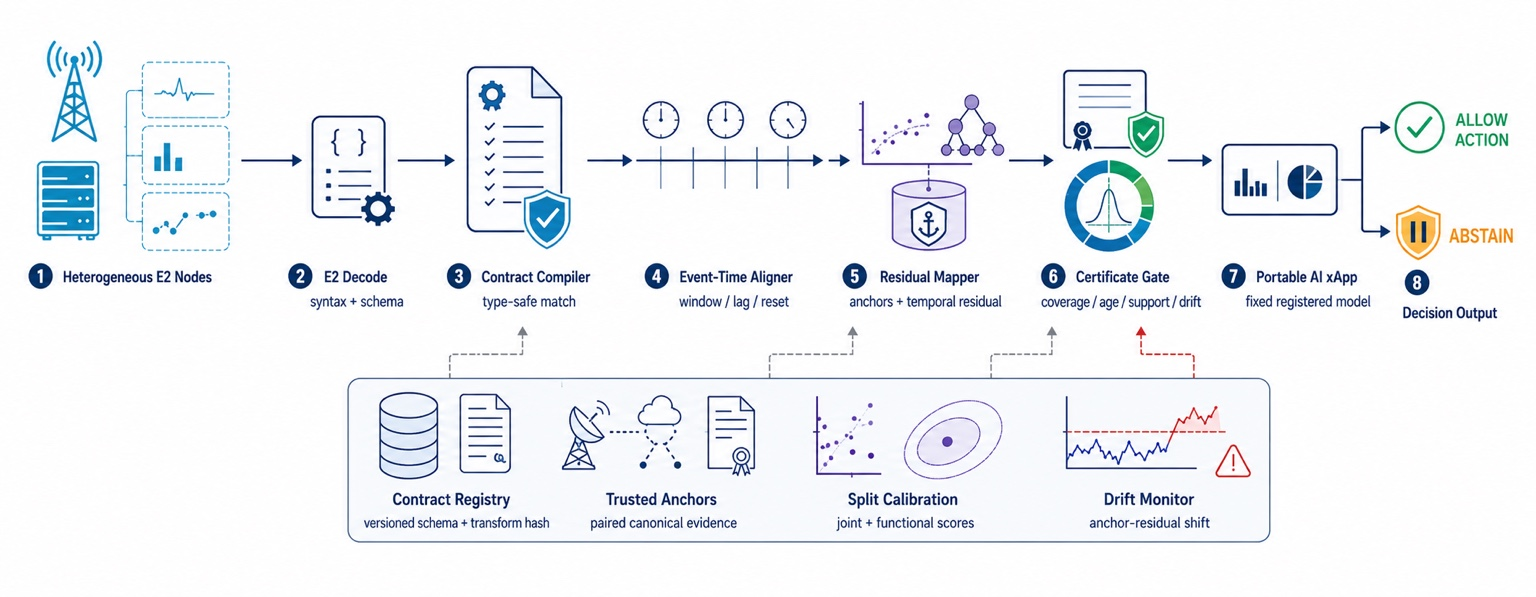
\includegraphics[width=\textwidth]{figures/fig1_kpm_bridge_architecture.jpeg}
\caption{KPM-Bridge placement between E2 decoding and a portable AI xApp. The data path compiles and aligns reports; the evidence plane supplies versioned contracts, trusted anchors, calibration, and drift state.}
\label{fig:architecture}
\end{figure*}

Figure~\ref{fig:architecture} places the bridge after E2 decoding and before the portable xApp feature interface. The fast path $y_{v,t}\mapsto(\hat z_t,\gamma_t)$ stays inside the Near-RT RIC and adds no radio control round trip. A slower evidence plane maintains $C_v$, paired anchors, calibration scores, and the current validity state of epoch $e$.

\subsection{Type-Safe Contract Compilation}
Let $C_v=\{c_{v,i}\}_{i=1}^{p_v}$ and $C^\star=\{c_k^\star\}_{k=1}^{d}$ be the source and target contract sets. The compiler constructs a bipartite graph $G_v=(C_v,C^\star,E_v)$. An edge $(i,k)$ exists only when quantity, physical dimension, and entity scope match; a missing edge is equivalent to cost $+\infty$. Every finite edge receives
\begin{equation}
\begin{aligned}
\kappa_{ik}={}&\beta_a\ind[a_i\ne a_k^\star]
+\beta_w\left|\log\frac{w_i}{w_k^\star}\right|_{[0,K_w]}\\
&+\beta_\tau\ind[\tau_i\ne\tau_k^\star]
+\beta_\rho\ind[\rho_i\ne\rho_k^\star].
\end{aligned}
\label{eq:semantic-cost}
\end{equation}
where $\boldsymbol\beta=(\beta_a,\beta_w,\beta_\tau,\beta_\rho)\in\R_+^4$ contains operator-set penalties. Since $w_i,w_k^\star>0$, the log-ratio is defined, and $|x|_{[0,K_w]}=\min\{|x|,K_w\}$ with $K_w>0$ prevents one window mismatch from dominating the matching objective. After type pruning, the compiler solves an injective matching $\pi_v:C^\star\hookrightarrow C_v$ minimizing $\sum_k\kappa_{\pi_v(k),k}$. Each selected edge emits unit/counter transforms, reset logic, clock/window obligations, and provenance binding. A window mismatch is not presumed invertible; it enlarges temporal and residual uncertainty. If $\pi_v(k)$ does not exist or $\kappa_{\pi_v(k),k}$ exceeds its budget, target $k$ fails closed.

\begin{figure*}[t]
\centering
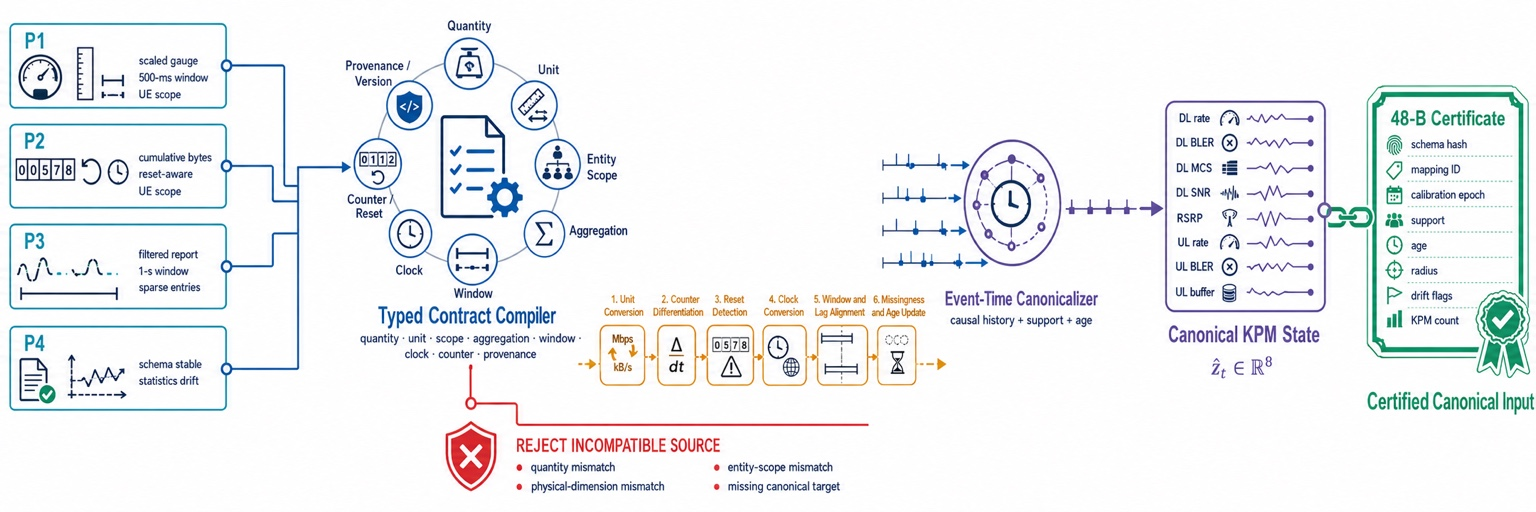
\includegraphics[width=\textwidth]{figures/fig2_typed_canonicalization.jpeg}
\caption{Typed canonicalization from heterogeneous KPM profiles to a certified eight-dimensional state. Incompatible quantities or scopes fail closed; compatible streams receive unit/counter transforms and explicit clock, window, and missingness obligations.}
\label{fig:semantic}
\end{figure*}

Figure~\ref{fig:semantic} visualizes the two-stage rule in \eqref{eq:semantic-cost} and Algorithm~\ref{alg:compiler}. Quantity, dimension, and scope determine the Boolean type predicate $T_{ik}\in\{0,1\}$; unit, counter, clock, and window differences affect $\kappa_{ik}$ only after $T_{ik}=1$. The red path is therefore a semantic rejection, not a low-confidence statistical prediction.

\begin{algorithm}[t]
\caption{Compilation of source KPM contracts into a type-safe canonical transform plan.}
\label{alg:compiler}
\footnotesize
\renewcommand{\arraystretch}{1.05}
\begin{tabular}{@{}r p{0.83\columnwidth}@{}}
\alghead{Input: authenticated registry records $C_v$, targets $C^\star$, per-target budgets, version $\nu$}
1 & Validate registry binding, mandatory fields, provenance, and schema versions.\\
2 & For each $(i,k)$, remove quantity, dimension, or scope mismatches; otherwise compute $\kappa_{ik}$ by \eqref{eq:semantic-cost}.\\
3 & Solve the minimum-cost injective assignment over finite edges.\\
4 & If any target is unmatched or exceeds its budget, return \textsc{unsupported} with a reason code.\\
5 & Emit target-ordered unit/counter transforms and clock/window obligations.\\
6 & Compute one Secure Hash Algorithm 256 (SHA-256) digest over the canonical serialization of $(C_v,C^\star,\text{plan},\nu)$ and its semantic budget; bind bytes 0--15 as the schema hash and bytes 16--23 as the mapping identifier.\\
\alghead{Output: executable transform plan, or a fail-closed reason code}
\end{tabular}
\end{algorithm}

The schema hash and mapping identifier are disjoint slices of one SHA-256 digest. This detail keeps the compiler, reference implementation, and fixed byte allocation in Table~\ref{tab:certificate} consistent.

\subsection{Event-Time Alignment and Residual Mapping}
The executable plan applies declared transforms before any learned correction. For a cumulative counter $b_t$ sampled after $\Delta_t>0$, the candidate rate is $r_t=(b_t-b_{t-1})/\Delta_t$. If $b_t-b_{t-1}<0$, the reset flag is raised. The alternative $r_t=b_t/\Delta_t$ is permitted only when reset metadata places the reset on the sampling boundary, as in the controlled profiles; otherwise $m_t^{(r)}=0$. Missing adjacent values are not extrapolated.

For each canonical instant, the reference implementation forms a causal design vector
\begin{equation}
x_t=[\tilde y_t,\tilde y_{t-1},\tilde y_{t-2},\tilde y_{t-4},\tilde y_{t-8},
\Delta\tilde y_t,m_t,\operatorname{age}_t,\operatorname{support}_t],
\label{eq:temporal-design}
\end{equation}
Here $\tilde y_t$ is the contract-normalized report, $\Delta\tilde y_t=\tilde y_t-\tilde y_{t-1}$ is causal, $m_t$ is the mask, and $(\operatorname{age}_t,\operatorname{support}_t)$ summarize event-time staleness and completeness. The lag set is $\mathcal L=\{0,1,2,4,8\}$, so no future report enters $x_t$. One histogram gradient-boosted regressor per coordinate predicts the standardized target \cite{friedman2001gradient}. The released mapper uses 70 trees, at most 15 leaves, depth five, and fixed seeds. This estimator is replaceable: the contract and certificate interfaces also admit linear, monotone, or neural residual maps. A temporal-ridge variant appears in the ablation.

\subsection{Joint and Functional Calibration}
On held-out samples $(\hat z_j,z_j)\in\mathcal D_v^C$, define the joint nonconformity score
\begin{equation}
R_j=\norm{D^{-1}(\hat z_j-z_j)}_2.
\label{eq:joint-score}
\end{equation}
For $n_c$ scores and $\alpha\in(0,1)$, let
\begin{equation}
\begin{aligned}
\hat q_\alpha&=R_{(\lceil(n_c+1)(1-\alpha)\rceil)},\\
\cU_t&=\{z:\norm{D^{-1}(z-\hat z_t)}_2\le\hat q_\alpha\}.
\end{aligned}
\label{eq:conformal-set}
\end{equation}
The convention $R_{(n_c+1)}=+\infty$ preserves validity when $\alpha<1/(n_c+1)$. Under exchangeability, \eqref{eq:conformal-set} is the standard split-conformal construction and gives $\Pr\{z_t\in\cU_t\}\ge1-\alpha$ \cite{vovk2022algorithmic,angelopoulos2023conformal}. A $d$-dimensional ball can nevertheless be conservative for one registered xApp, so KPM-Bridge separately calibrates
\begin{equation}
\begin{aligned}
S_j&=|\ell(\hat z_j)-\ell(z_j)|,\\
\hat q_\alpha^\ell&=S_{(\lceil(n_c+1)(1-\alpha)\rceil)},\\
I_t^\ell&=[\ell(\hat z_t)-\hat q_\alpha^\ell,\ell(\hat z_t)+\hat q_\alpha^\ell].
\end{aligned}
\label{eq:functional-set}
\end{equation}
The functional interval supplements rather than replaces $\cU_t$. It is bound to the registered model hash, so changing $\ell$ invalidates $I_t^\ell$. The authenticated registry resolves $(\ell,\hat q_\alpha^\ell,\theta,a_{\max},s_{\min})$ from the mapping identifier and calibration epoch; the compact sidecar need not repeat the fixed quantile. The guarantees $\Pr\{z_t\in\cU_t\}\ge1-\alpha$ and $\Pr\{\ell(z_t)\in I_t^\ell\}\ge1-\alpha$ are marginal. Simultaneous coverage requires multiplicity correction or a joint score.

\emph{Drift invalidation and admission:}
Trusted anchors periodically reveal standardized residuals $r_t=D^{-1}(\hat z_t-z_t)\in\R^d$. Calibration anchors estimate $(\mu_r,\Sigma_r)$. For a window of $W=5$ anchors, the monitor evaluates
\begin{equation}
H_t=\sqrt{W(\bar r_t-\mu_r)^\top(\Sigma_r+0.1I)^{-1}(\bar r_t-\mu_r)}.
\label{eq:drift-score}
\end{equation}
where $\bar r_t=W^{-1}\sum_{j=0}^{W-1}r_{t-j}$ and $0.1I_d$ regularizes the covariance. Anchors arrive every ten samples, or 2.5~s in this corpus. The alarm threshold $h_{.975}$ is the 97.5th percentile of the \emph{per-stream maximum} calibration statistic, which accounts for repeated tests more directly than a pointwise quantile. Candidate $W$ values are ranked without test data on held-out \texttt{exp1} streams under a predeclared 5\% validation false-alarm ceiling and synthetic 1.25-scale shifts; this selects $W=5$. If $H_t>h_{.975}$, the epoch is invalidated rather than the stale interval widened. Recalibration is a separate control-plane operation.

\begin{algorithm}[t]
\caption{Certified streaming inference with event-time alignment, calibrated uncertainty, drift checks, and selective action.}
\label{alg:stream}
\footnotesize
\renewcommand{\arraystretch}{1.05}
\begin{tabular}{@{}r p{0.83\columnwidth}@{}}
\alghead{Input: report/metadata, compiled plan, mapper, calibration epoch, quality budgets}
1 & Verify schema hash, mapping identifier, source provenance, and epoch.\\
2 & Apply unit/counter transforms, enforce clock/window obligations, and update \eqref{eq:temporal-design}.\\
3 & Predict $\hat z_t$ and attach $\hat q_\alpha$, support, age, and calibration epoch.\\
4 & At an anchor, update $H_t$ by \eqref{eq:drift-score}; invalidate the epoch on a trigger.\\
5 & Compute $I_t^\ell$ by \eqref{eq:functional-set} and evaluate support, age, drift, and threshold crossing.\\
6 & Serialize the 48-byte certificate; emit the xApp action if admitted, else \textsc{abstain} with a reason code.\\
\alghead{Output: canonical vector, certificate, action/abstention, and reason code}
\end{tabular}
\end{algorithm}

Algorithm~\ref{alg:stream} is the online counterpart of Algorithm~\ref{alg:compiler}. Its admission predicate is the conjunction
\begin{equation}
\begin{aligned}
G_t=\ind\{&\operatorname{age}_t\le a_{\max},
\operatorname{support}_t\ge s_{\min},\ H_t\le h_{.975},\\
&\theta\notin I_t^\ell,\ \gamma_t\ \text{valid}\}.
\end{aligned}\label{eq:admission-gate}
\end{equation}
Thus the temporal design in \eqref{eq:temporal-design}, functional interval in \eqref{eq:functional-set}, and drift statistic in \eqref{eq:drift-score} meet in one auditable decision: act if $G_t=1$, otherwise abstain with a reason code.

The encoded sidecar is fixed at \CertificateBytes: 16 bytes for the schema hash, $2\times8$ bytes for mapping and calibration identifiers, $3\times4$ bytes for support, age, and generic radius, and $2\times2$ bytes for flags and KPM count. The authenticated registry supplies the functional quantile, while the canonical vector is carried separately.

\subsection{O-RAN Placement and Certificate Lifecycle}
KPM-Bridge is an internal evidence layer, not a replacement for the E2 Application Protocol (E2AP) or E2SM-KPM. E2 termination handles subscription and Abstract Syntax Notation One decoding, then forwards values and metadata to the local adapter. The lookup key $(\mathrm{E2Node},\mathrm{E2SMRev},\mathrm{MeasID},\mathrm{PolicyID})$ selects the contract. Service Management and Orchestration or the non-real-time RIC (Non-RT RIC) may provision the registry, but no new standardized A1, O1, or R1 message is claimed. The xApp-facing API returns $(\hat z_t,\gamma_t,\mathrm{reason}_t)$.

\begin{figure*}[t]
\centering
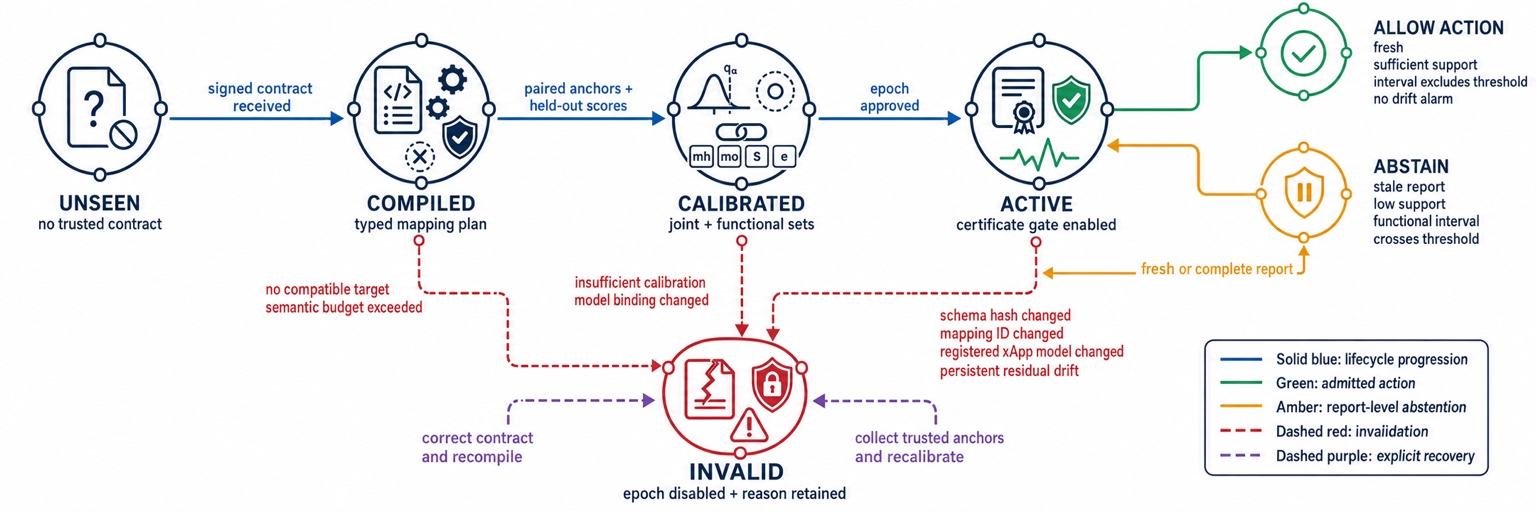
\includegraphics[width=\textwidth]{figures/fig3_certificate_lifecycle.jpeg}
\caption{Certificate lifecycle from an unseen contract to an active or invalid state. Schema or model changes force recompilation, whereas statistical drift requires new trusted anchors and recalibration.}
\label{fig:lifecycle}
\end{figure*}

Figure~\ref{fig:lifecycle} defines the persistent state machine $L_e\in\{\textsc{Unseen},\textsc{Compiled},\textsc{Calibrated},\textsc{Active},\textsc{Invalid}\}$. \textsc{Unseen} has no signed contract. \textsc{Compiled} has a valid type match and transform plan but no statistical guarantee. \textsc{Calibrated} binds $(M_v,D,\hat q_\alpha,\hat q_\alpha^\ell,\mu_r,\Sigma_r)$ to epoch $e$. \textsc{Active} may evaluate $G_t$. \textsc{Invalid} is fail closed and retains its reason; it never transitions automatically to \textsc{Active}. A schema change returns to compilation, while a residual alarm requires new anchors and calibration.

\begin{table}[t]
\caption{Fixed 48-byte certificate layout and the operational meaning of each field.}
\label{tab:certificate}
\centering
\scriptsize
\setlength{\tabcolsep}{3.2pt}
\begin{tabular}{lrl}
\toprule
Field & Bytes & Purpose \\
\midrule
Schema hash & 16 & binds source, target, and plan \\
Mapping identifier & 8 & selects fitted mapper \\
Calibration epoch & 8 & invalidation boundary \\
Support & 4 & observed KPM fraction \\
Age & 4 & event-time staleness in ms \\
Radius & 4 & generic conformal radius \\
Flags & 2 & drift/schema/quality bits \\
KPM count & 2 & canonical dimension guard \\
\midrule
Total & 48 & network byte order \\
\bottomrule
\end{tabular}
\end{table}

Serialization uses network byte order and fixed-width fields. The 16-byte hash is a compact truncated digest, not a digital signature; registry updates must be authenticated by the RIC platform. Mapping and epoch identifiers prevent the invalid combination $(\hat z_t^{(e)},I_t^{\ell,(e')})$ with $e\neq e'$. Floating-point support, age, and radius are adequate for the reference implementation, while a safety-critical deployment may specify fixed point under a new layout version.

Table~\ref{tab:certificate} accounts for all $16+8+8+4+4+4+2+2=48$ bytes. The object is a local evidence sidecar; $\hat z_t$ remains a separate payload.

\begin{table*}[t]
\caption{Fail-closed conditions, emitted reason codes, and required recovery actions.}
\label{tab:failures}
\centering
\scriptsize
\setlength{\tabcolsep}{5pt}
\begin{tabular}{llll}
\toprule
Condition & Observable evidence & Immediate action & Recovery \\
\midrule
Quantity/dimension/scope mismatch & no finite compiler edge & reject mapping & correct contract or source KPM \\
Unknown reset or adjacent counter loss & invalid delta and reduced support & mark feature missing & next valid delta or anchor \\
Schema/model hash change & certificate binding mismatch & invalidate epoch & recompile and recalibrate \\
Age or support budget violation & $\operatorname{age}_t>a_{\max}$ or $\operatorname{support}_t<s_{\min}$ & abstain with reason & fresh/complete report \\
Functional interval crosses threshold & $\theta\in I_t^\ell$ & abstain & refine, wait, or operator policy \\
Anchor-residual mean shift & $H_t$ exceeds stream threshold & invalidate epoch & diagnose and recalibrate \\
\bottomrule
\end{tabular}
\end{table*}

Reason codes separate $\mathrm{unsupported}$ from $\mathrm{uncertain}$. More samples cannot repair $T_{ik}=0$, whereas a type-compatible stream may recover after a fresh report or anchor. Table~\ref{tab:failures} maps each predicate failure to a fail-closed action and a distinct recovery path, preventing an orchestrator from repeatedly refining a fundamentally incompatible KPM.

\section{Analytical Guarantees}
\begin{proposition}[Compiler type soundness]
If Algorithm~\ref{alg:compiler} returns a mapping, every selected source and target have equal quantity, physical dimension, and entity scope.
\end{proposition}
\begin{IEEEproof}
An edge is inserted only after all three equality predicates pass. The assignment solver selects only finite inserted edges. Therefore every returned pair satisfies the predicates. Unit, temporal, and counter differences may remain, but they are explicit transforms rather than silent type substitutions.
\end{IEEEproof}

Type soundness is necessary but not sufficient for identifiability. A cell mean cannot generally recover a per-UE vector, even when both are expressed in Mbit/s, so $T_{ik}=0$ rejects that scope change. By contrast, one-second and 250-ms means may satisfy $T_{ik}=1$ while carrying unequal information. Their edge is admissible only with an explicit window transform and residual uncertainty.

\begin{proposition}[Translation-error decomposition]
Unless a subscript states otherwise, the norms in this proposition are Euclidean.
Let $u_t^0$ be the noise-free, full-support output of the declared transform; $u_t^m$ its masked version; and $u_t^\epsilon$ the noisy masked input. Let $F_v^0$ be the fitted calibration-regime realization of $M_v$, and let $\bar z_t^0$ and $\bar z_t$ be the information-preserving targets under the calibration and current regimes. Then $\hat z_t=F_v^0(u_t^\epsilon)$ obeys
\begin{equation}
\begin{aligned}
\norm{\hat z_t-z_t}\le{}&E_{\rm temp}(t)+E_{\rm model}(t)+E_{\rm noise}(t)\\
&+E_{\rm miss}(t)+E_{\rm drift}(t),
\end{aligned}
\label{eq:error-decomposition}
\end{equation}
where $E_{\rm noise}=\norm{F_v^0(u_t^\epsilon)-F_v^0(u_t^m)}$, $E_{\rm miss}=\norm{F_v^0(u_t^m)-F_v^0(u_t^0)}$, $E_{\rm model}=\norm{F_v^0(u_t^0)-\bar z_t^0}$, $E_{\rm drift}=\norm{\bar z_t^0-\bar z_t}$, and $E_{\rm temp}=\norm{\bar z_t-z_t}$.
\end{proposition}
\begin{IEEEproof}
Insert $F_v^0(u_t^m)$, $F_v^0(u_t^0)$, $\bar z_t^0$, and $\bar z_t$ between $\hat z_t$ and $z_t$, then apply the triangle inequality. Compiler soundness removes a dimension/scope substitution term but not temporal or information-loss terms.
\end{IEEEproof}

\begin{proposition}[Non-identifiability under aggregation]\label{prop:nonident}
Suppose a source reports only $y=A z$, where $A$ is a linear aggregation operator, and there exist $z^{(1)}\ne z^{(2)}$ in the admissible state space with $Az^{(1)}=Az^{(2)}$. For any deterministic point mapper $M(y)$, at least one of the two states has
\begin{equation}
\norm{M(y)-z^{(j)}}_2\ge \tfrac{1}{2}\norm{z^{(1)}-z^{(2)}}_2.
\label{eq:impossibility}
\end{equation}
\end{proposition}
\begin{IEEEproof}
Both states generate the same report and therefore the same estimate. If both errors were smaller than half their separation, the triangle inequality would imply $\norm{z^{(1)}-z^{(2)}}_2<\norm{z^{(1)}-z^{(2)}}_2$, a contradiction.
\end{IEEEproof}

Proposition~\ref{prop:nonident} quantifies the information that no mapper can recover: if $z^{(1)}-z^{(2)}\in\ker(A)$, both states produce the same $y$, and at least one point error is half their separation. Anchors or structural priors may choose among such states, but that dependence must be bound to the mapping identifier and uncertainty set. The scope predicate rejects the clearest version of this failure before fitting begins.

\begin{assumption}[Calibration exchangeability]
Conditional on a fixed schema, mapping, model, and non-drift regime, the test score and the $n_c$ calibration scores are exchangeable. Calibration data are not used to fit the mapper.
\end{assumption}

\begin{proposition}[Finite-sample coverage]
Under calibration exchangeability, the set in \eqref{eq:conformal-set} satisfies
\begin{equation}
\Pr\{z_{n_c+1}\in\cU_{n_c+1}\}\ge 1-\alpha.
\label{eq:coverage}
\end{equation}
The functional interval in \eqref{eq:functional-set} obeys the analogous inequality for $\ell(z)$.
\end{proposition}
\begin{IEEEproof}
The rank of the test nonconformity score among $n_c+1$ exchangeable scores is uniform up to ties. The order statistic in \eqref{eq:conformal-set} excludes at most an $\alpha$ fraction of ranks. Applying the same argument to $S_j$ gives functional coverage \cite{vovk2022algorithmic,angelopoulos2023conformal}.
\end{IEEEproof}

Radio traces are temporally dependent. The experiment separates repetitions and subsamples calibration points, but Proposition 4 remains conditional on exchangeability of $(R_1,\ldots,R_{n_c+1})$. Section~\ref{sec:results} therefore reports measured coverage under the implemented split rather than extending \eqref{eq:coverage} to arbitrary autocorrelation.

\begin{proposition}[Decision stability]
For a threshold action $a(z)=\ind[\ell(z)\ge\theta]$, if $\theta\notin I_t^\ell$ and $\ell(z_t)\in I_t^\ell$, then $a(\hat z_t)=a(z_t)$. Under calibration exchangeability, the joint probability of passing the interval gate and disagreeing with the canonical action is at most $\alpha$; no conditional selective-error bound is claimed.
\end{proposition}
\begin{IEEEproof}
When $I_t^\ell$ lies strictly above or below $\theta$, all contained values induce the same action. Functional coverage gives
$\Pr\{\theta\notin I_t^\ell,\,a(\hat z_t)\ne a(z_t)\}\le\alpha$.
Support, age, and drift filters preserve this joint bound because they only remove events. They do not imply the conditional bound $\Pr\{a(\hat z_t)\ne a(z_t)\mid\text{admit}\}\le\alpha$; selective error is therefore measured separately.
\end{IEEEproof}

For a general utility $J:\cA\times\cZ\to\R$, a set-valued xApp can instead choose
\begin{equation}
a_t^\star\in\arg\max_{a\in\cA}\min_{z\in\cU_t}J(a,z),
\label{eq:robust-action}
\end{equation}
following the robust-optimization principle \cite{bertsimas2004robustness}. The evaluated binary risk xApp uses $I_t^\ell$, because the interval is tailored to its registered threshold $a(z)=\ind\{\ell(z)\ge\theta\}$.

For complexity, let $n_{\rm asn}=p_v+d$ be the padded assignment size, $h=\dim(x_t)$, $N_{\rm tr}$ the trees per coordinate, $L_{\rm tr}$ their maximum depth, $N_{\rm leaf}\le2^{L_{\rm tr}}$ their maximum leaves, and $W$ the drift window. Dense matching costs $O(n_{\rm asn}^3)$ time and $O(p_vd)$ memory, but runs only after a schema change. Per report, declared transforms and feature updates cost $O(hd)$, tree inference $O(dN_{\rm tr}L_{\rm tr})$, and set construction $O(d)$. At an anchor epoch, $H_t$ costs $O(d^2+Wd)$. Persistent model storage is $O(dN_{\rm tr}N_{\rm leaf})$. Once $(\hat q_\alpha,\hat q_\alpha^\ell,\mu_r,\Sigma_r)$ are materialized, online cost is independent of $n_c$.

\section{Experimental Design}
\subsection{Trace Backbone and Controlled Profiles}
The benchmark pins public ColO-RAN commit \texttt{bd86629} \cite{polese2023coloran}. Its Rome-static-medium scenario contains seven base stations (BSs), 42 UEs, 10~MHz bandwidth, 50 physical resource blocks (PRBs), and enhanced mobile broadband (eMBB), machine-type communication (MTC), and ultra-reliable low-latency communication (URLLC) slices. Round-robin, water-filling, and proportional-fair schedulers span 28 resource allocations.

The deterministic subset is the Cartesian cross of three schedulers, configurations $\{\texttt{tr0},\texttt{tr9},\texttt{tr18}\}$, experiments $\{\texttt{exp1},\texttt{exp2}\}$, BS1/BS4, and one UE per traffic class. It contains 108 files and 208,585 raw rows. A predeclared rule excludes two traces with fewer than 400 attached samples. After removing the four-sample prediction horizon, 53 \texttt{exp1} traces (\TrainingRows\ rows) form the fitting/calibration source and 53 independent \texttt{exp2} traces (\TestRows\ rows) form the test set. Every file is hash verified; GNU General Public License version 3.0 (GPL-3.0) data are fetched from upstream rather than redistributed.

The canonical vector is $z_t=(R_t^{\rm DL},B_t^{\rm DL},M_t^{\rm DL},S_t^{\rm DL},P_t^{\rm RSRP},R_t^{\rm UL},B_t^{\rm UL},Q_t^{\rm UL})\in\R^8$: reported downlink (DL) rate, DL block error rate (BLER), DL modulation and coding scheme (MCS), DL signal-to-noise ratio (SNR), reference signal received power (RSRP), uplink (UL) rate, UL BLER, and UL buffer. These names follow dataset fields; source units are not relabelled as standardized commercial KPMs.


\begin{table*}[t]
\caption{Controlled implementation profiles applied to the public traces.}
\label{tab:profiles}
\centering
\scriptsize
\setlength{\tabcolsep}{4.2pt}
\begin{tabular}{llllllll}
\toprule
Profile & Declared representation & Window & Lag & Entry loss & Noise & Quantization & Additional condition \\
\midrule
P1 & scaled units / gauges & 2 samples & 1 sample & 3\% & 2\% & 1\% & mild hidden filter \\
P2 & rates as resetting counters & 3 samples & 1 sample & 8\% & 3\% & 1.5\% & resets every 257 samples \\
P3 & scaled units / gauges & 4 samples & 2 samples & 18\% & 5\% & 3\% & sparse filtered reports \\
P4 & scaled units / gauges & 2 samples & 1 sample & 5\% & 2.5\% & 1.2\% & shift at 55\% of each test trace \\
\bottomrule
\end{tabular}
\end{table*}


\emph{Controlled implementation profiles:}
Profiles P1--P4 in Table~\ref{tab:profiles} are deterministic maps $\Psi_p:z_{1:T}\mapsto y_{p,1:T}$ applied to each real trace. They vary scale, unit representation, window, lag, training-scale noise, entry loss, burst loss, quantization, hidden monotone filtering, and reset semantics. P4 changes at $t_s=0.55T$ through a persistent 1.25-standard-scale offset, a smaller nonlinear gain change, doubled noise, and two extra lag samples. No profile is attributed to a vendor.

P0 is an identity reference with 0.2\% noise and is used only for software checks. P1--P3 test stationary portability, whereas P4 tests invalidation under severe unannounced drift. The global seed is 20,260,712 and each profile seed is a stable hash of $(p,\mathrm{traceID})$.

\subsection{xApp, Baselines, and Metrics}
The fixed xApp predicts one-second quality-of-service (QoS) risk from $z_t$. For each traffic class, label $Y_t^{\rm risk}=1$ when the next-four-sample mean DL rate is below its training-only 35th percentile or BLER exceeds its training-only 75th percentile. Thresholds, feature statistics, and the class-balanced logistic model use only the first $0.6T$ samples of each canonical \texttt{exp1} trace; the four-sample horizon is removed at the boundary. The registered functional is the fitted logit
\begin{equation}
\ell(z)=w^\top\!\left[(z-\mu_x)\oslash\sigma_x\right]+b,
\label{eq:xapp-logit}
\end{equation}
where $(w,b)$ are logistic parameters, $(\mu_x,\sigma_x)$ are fit-prefix feature location and scale, and $\oslash$ is elementwise division. On canonical \texttt{exp2}, the instrument has area under the receiver-operating-characteristic curve (AUROC) 0.755, Brier score 0.205, and prevalence 44.9\%. These quantities characterize the fixed xApp; KPM-Bridge does not alter its intrinsic accuracy.

With intervention cost $c_a=.2$ and missed-risk cost $c_m=1$, the probability threshold is $c_a/c_m=.2$. Equivalently, \eqref{eq:functional-set} uses $\theta=\log(.2/.8)\simeq-1.386$ with \eqref{eq:xapp-logit}. Clairvoyant-label regret is $.8$ for a miss and $.2$ for an unnecessary action. Agreement with the \emph{same} xApp on canonical $z_t$ is the primary portability measure, which separates telemetry translation error from source-model error.

\emph{Fitting and calibration:}
For each \texttt{exp1} trace, the first 60\% is the fitting prefix and 10\% of that prefix becomes evenly spaced paired anchors. The remaining 40\% is excluded from fitting; every fourth sample enters $\mathcal D_v^C$. The full \texttt{exp2} repetition is untouched test data. Gradient-boosting hyperparameters are fixed across profiles.

The seven portable baselines are direct input with median fill, contract conversion, featurewise z-score alignment, CORAL \cite{sun2016deepcoral}, Gaussian OT \cite{courty2017ot,peyre2019optimal}, supervised current-sample anchor ridge, and temporal ridge. Two bounds are also reported: deployment-specific logistic retraining on the 60\% prefixes and oracle canonical input. Retraining is not portable and uses roughly ten times more task labels than the bridge uses mapping anchors.

Distribution baselines receive the same anchor-budget samples but not their eventwise pairing. With raw moments $(\mu_y,C_y)$ and canonical moments $(\mu_z,C_z)$, z-score alignment is featurewise, while CORAL and Gaussian OT use
\begin{equation}
\begin{aligned}
T_{\rm CORAL}(y)&=(y-\mu_y)C_y^{-1/2}C_z^{1/2}+\mu_z,\\
T_{\rm OT}(y)&=(y-\mu_y)C_y^{-1/2}
(C_y^{1/2}C_zC_y^{1/2})^{1/2}C_y^{-1/2}+\mu_z.
\end{aligned}
\label{eq:baselines}
\end{equation}
Both transforms use covariance regularization $10^{-5}I_d$. Anchor ridge is multivariate and supervised but receives only $y_t$; temporal ridge receives the same $x_t$ as KPM-Bridge. The comparison therefore separates nonlinear residual capacity from temporal context and semantic preprocessing without withholding available history.

\begin{table}[t]
\caption{Information and supervision made available to each evaluated method family.}
\label{tab:fairness}
\centering
\scriptsize
\setlength{\tabcolsep}{3pt}
\begin{tabular}{lccc}
\toprule
Method family & Contracts & Paired anchors & Task labels \\
\midrule
Direct / distribution & no & no & no \\
Contract only & yes & no & no \\
Anchor/temporal ridge & yes & 10\% & no \\
KPM-Bridge & yes & 10\% & no \\
Deployment retrain & no & no & 60\% fit prefix \\
Oracle canonical & canonical & n/a & source model \\
\bottomrule
\end{tabular}
\end{table}

Table~\ref{tab:fairness} prevents two misleading comparisons. Distribution alignment is cheaper because it is unsupervised, but it has no paired correctness signal. Deployment retraining solves a different problem: it consumes local task labels and replaces the xApp parameters $(w,b)$. Its performance is therefore not evidence that the original model is portable.

Pooled canonical error is $\mathrm{NRMSE}=\sqrt{\E\|D^{-1}(\hat z-z)\|_2^2/d}$. Additional metrics include normalized absolute error, fixed-xApp agreement, label regret, joint coverage, radius, acceptance $A_{\rm acc}=\Pr\{G_t=1\}$, conditional disagreement $E_{\rm sel}=\Pr\{\hat a_t\neq a_t^\star\mid G_t=1\}$, and joint exposure $J_{\rm exp}=A_{\rm acc}E_{\rm sel}$, plus missed-risk rate, drift detection/delay, trace false alarm, fit time, amortized inference, and serialized bytes. Every 95\% interval resamples whole test traces 1,000 times, so no row-level independence is assumed. Runtime uses one Open Multi-Processing (OpenMP)/Basic Linear Algebra Subprograms (BLAS) thread.

\begin{table}[t]
\caption{Fixed data split, calibration, model, and execution controls used for reproducibility.}
\label{tab:repro}
\centering
\scriptsize
\setlength{\tabcolsep}{3.2pt}
\begin{tabular}{ll}
\toprule
Item & Fixed value \\
\midrule
Upstream revision & \texttt{bd86629d07d5} \\
Global seed & 20,260,712 \\
Mapper fit region & first 60\% of \texttt{exp1} \\
Paired anchors & 10\% of fit region \\
Calibration & last 40\%, stride four \\
Conformal level & $\alpha=0.05$ unless swept \\
Residual model & 70 trees/KPM, depth five \\
Drift anchors & every 10 samples; $W=5$ \\
Bootstrap & 1,000 whole-trace resamples \\
Threads & one OpenMP/BLAS thread \\
\bottomrule
\end{tabular}
\end{table}

Every generated result carries a status distinguishing the full benchmark from the smoke test. Tables and numerical macros are produced from comma-separated outputs, and a fail-closed audit checks the remaining prose values against the same files. The manifest stores SHA-256 and byte count for every upstream input. Table~\ref{tab:repro} fixes the split, seed, calibration level, model capacity, and execution environment.

\section{Results}\label{sec:results}
\subsection{Stationary Cross-Implementation Portability}
\begin{figure}[t]
\centering
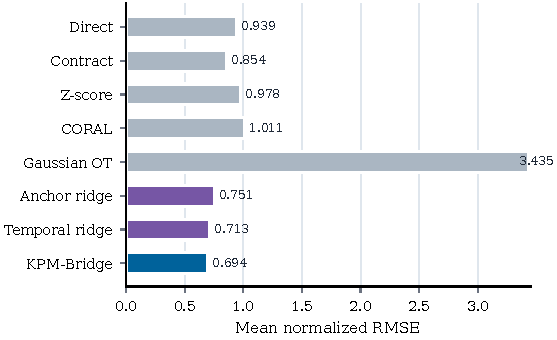
\includegraphics[width=\columnwidth]{figures/fig_stationary_nrmse.pdf}
\caption{Stationary normalized reconstruction error across profiles P1--P3 for all portable methods. Lower values indicate more accurate canonical KPM recovery.}
\label{fig:stationary-nrmse}
\end{figure}

\begin{figure}[t]
\centering
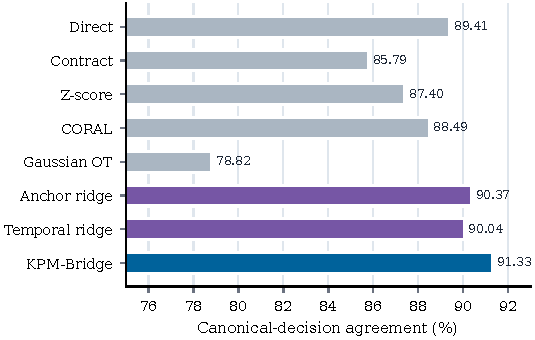
\includegraphics[width=\columnwidth]{figures/fig_stationary_agreement.pdf}
\caption{Fixed-xApp decision agreement across stationary profiles P1--P3. Higher values indicate closer agreement with decisions made from canonical inputs.}
\label{fig:stationary-agreement}
\end{figure}


\begin{table}[t]
\caption{Mean performance across stationary profiles P1--P3.}
\label{tab:main}
\centering
\scriptsize
\setlength{\tabcolsep}{3.2pt}
\begin{tabular}{lrrrr}
\toprule
Method & NRMSE$\downarrow$ & Agree (\%)$\uparrow$ & Regret$\downarrow$ & $\mu$s/sample \\
\midrule
Direct & 0.923 & 89.41 & 0.1079 & 0.02 \\
Contract & 3.210 & 85.79 & 0.1138 & 0.26 \\
Z-score & 0.961 & 87.40 & 0.1029 & 0.04 \\
CORAL & 0.994 & 88.49 & 0.1013 & 0.04 \\
Gaussian OT & 2.917 & 78.82 & 0.1263 & 0.04 \\
Anchor ridge & 0.752 & 90.37 & 0.1031 & 0.52 \\
Temporal ridge & 0.717 & 90.04 & 0.1029 & 1.20 \\
\textbf{KPM-Bridge} & \textbf{0.685} & \textbf{91.33} & \textbf{0.0980} & \textbf{22.12} \\
\bottomrule
\end{tabular}
\end{table}


Figures~\ref{fig:stationary-nrmse} and \ref{fig:stationary-agreement} and Table~\ref{tab:main} summarize P1--P3. KPM-Bridge attains $\overline{\mathrm{NRMSE}}=$\StableNrmse, an observed \NrmseGainBest\ reduction from temporal ridge, the strongest reconstruction baseline. Fixed-xApp agreement is \StableAgreement, or \AgreementGainBest\ above the strongest decision baseline. Mean label regret is 0.0977, compared with 0.1033 for CORAL and 0.1019 for temporal ridge. Because the whole-trace intervals overlap, these are descriptive differences rather than significance claims.

For P1--P3, the profile vector is $\boldsymbol e=(.675,.682,.725)$ with whole-trace bootstrap 95\% intervals $[.600,.749]$, $[.607,.759]$, and $[.636,.817]$. Their width exposes trace heterogeneity that row-level resampling would suppress. Agreement ranges from 87.94\% to 90.13\%.

P2 explains much of the separation. Contract-only differentiation forms $r_t=(b_t-b_{t-1})/\Delta_t$; a missing neighbor makes $r_t$ unavailable, while counter noise and quantization are amplified by the difference. Anchor ridge reduces the error, and temporal models use history plus $m_t$. Gaussian OT degrades because matching the marginal law of $b_t$ to that of $r_t$ cannot reconstruct eventwise increments. Distribution alignment cannot replace counter semantics.

Direct input still obtains 87.81\% agreement despite poor reconstruction because the canonical xApp acts on 88.66\% of test samples. With such class imbalance, a high agreement can coexist with large $\|D^{-1}(\hat z-z)\|_2$. NRMSE, regret, and selective disagreement are therefore interpreted jointly.

\subsection{Featurewise Error Structure}
\begin{figure}[t]
\centering
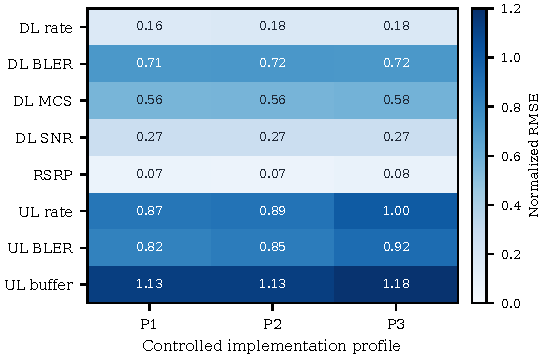
\includegraphics[width=\columnwidth]{figures/fig_feature_nrmse.pdf}
\caption{Per-KPM normalized reconstruction error for KPM-Bridge across profiles P1--P3, exposing feature-level variation hidden by the pooled metric.}
\label{fig:feature-nrmse}
\end{figure}

\begin{figure}[t]
\centering
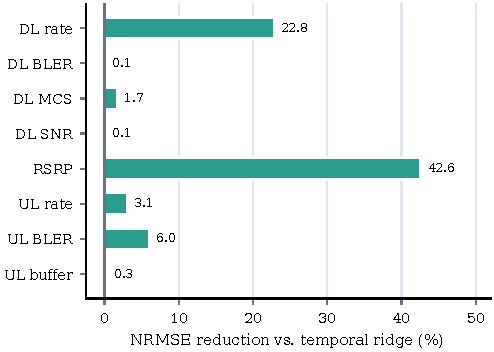
\includegraphics[width=\columnwidth]{figures/fig_feature_gain.pdf}
\caption{Featurewise NRMSE reduction relative to temporal ridge. Positive values indicate lower reconstruction error for KPM-Bridge.}
\label{fig:feature-gain}
\end{figure}

Figures~\ref{fig:feature-nrmse} and \ref{fig:feature-gain} expose what the pooled norm hides. DL-rate NRMSE lies in $[.162,.176]$, and RSRP remains below .080. UL buffer is hardest, $[1.13,1.18]$, because its distribution is zero-inflated with rare bursts; UL rate and BLER are also more variable than their DL counterparts. Relative to temporal ridge, the nonlinear residual lowers mean DL-rate error by 22.8\% and RSRP error by 42.6\%, but changes DL-BLER error by only 0.108\%. The gain $G_k=1-e_k^{\rm bridge}/e_k^{\rm ridge}$ is thus feature dependent: nonlinear scaling and saturation benefit, whereas sparse bursts remain anchor limited.

This feature structure also explains why agreement improves less than NRMSE. In \eqref{eq:xapp-logit}, the dominant coordinates are DL rate and DL BLER. KPM-Bridge materially improves the former but not the latter; RSRP and UL improvements perturb $\ell(z)$ only through smaller coefficients $w_k$. Another xApp, with $w'\neq w$, would require a different functional certificate and could value the same reconstruction errors differently.

\subsection{Calibration and Selective Inference}

\begin{table}[t]
\caption{Calibration, selective inference, and drift outcomes at $\alpha=0.05$.}
\label{tab:selective}
\centering
\scriptsize
\setlength{\tabcolsep}{2.6pt}
\begin{tabular}{lrrrrrr}
\toprule
Profile & Cov. (\%) & Accept (\%) & Sel. err. (\%) & Wilson hi. & Detect (\%) & Delay (s) \\
\midrule
P1 & 94.06 & 57.37 & 0.200 & 0.242 & -- & -- \\
P2 & 94.48 & 54.89 & 0.276 & 0.326 & -- & -- \\
P3 & 94.51 & 48.33 & 0.222 & 0.270 & -- & -- \\
P4 & 94.47 & 34.49 & 5.393 & 5.646 & 90.6 & 8.96 \\
\bottomrule
\end{tabular}
\end{table}


Across P1--P3 at $\alpha=.05$, Table~\ref{tab:selective} gives empirical joint coverage \StableCoverage, 0.68 percentage points below $1-\alpha=.95$. Experiment-level separation removes shared repetitions, but temporal dependence makes exchangeability approximate. The mean generic radius is $\overline q_{.05}=3.324$ training scales.

For the registered logit, $I_t^\ell$ is more selective than the generic $d$-ball. Mean acceptance is $A_{\rm acc}=$\StableAcceptance\ and conditional canonical-action disagreement is $E_{\rm sel}=$\StableSelectiveError. Per-profile whole-trace upper limits are .403\%, .361\%, and .352\%; none supports a zero-error claim. Removing $\hat q_\alpha^\ell$ increases $E_{\rm sel}$ to 9.67--11.73\% while increasing $A_{\rm acc}$ to 78.10--92.18\%.

\begin{figure}[t]
\centering
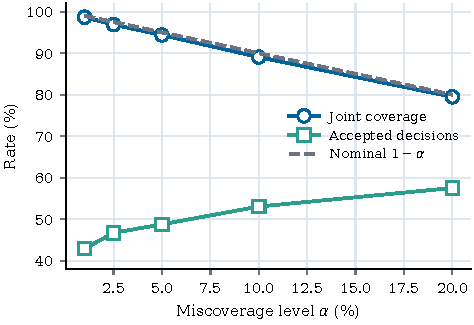
\includegraphics[width=\columnwidth]{figures/fig_coverage_availability.pdf}
\caption{Empirical joint coverage and accepted-decision rate versus conformal miscoverage level $\alpha$. The dashed line is the nominal coverage target $1-\alpha$.}
\label{fig:coverage-availability}
\end{figure}

\begin{figure}[t]
\centering
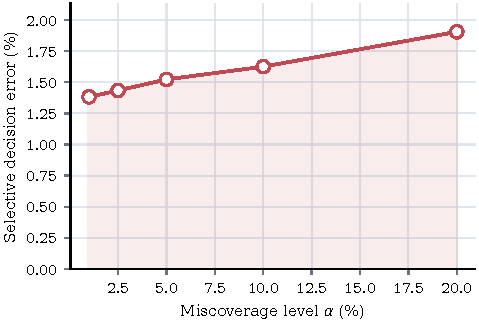
\includegraphics[width=\columnwidth]{figures/fig_selective_error.pdf}
\caption{Mean conditional canonical-action disagreement versus conformal miscoverage $\alpha$ across profiles P1--P4.}
\label{fig:selective-error}
\end{figure}

Figures~\ref{fig:coverage-availability} and \ref{fig:selective-error} sweep $(\hat q_\alpha,\hat q_\alpha^\ell)$. As $\alpha:.01\to.20$, mean P1--P4 coverage changes $98.72\%\to79.15\%$, acceptance $44.41\%\to56.96\%$, and conditional disagreement $1.51\%\to1.94\%$. The curves describe a three-way tradeoff among coverage, availability, and error; they do not determine a universal $\alpha$.

\subsection{Drift Invalidation}
Before the P4 shift, empirical coverage is 94.43\%. At 1.25 training scales, the residual monitor detects \DriftDetection\ of traces with \DriftDelay\ median delay and \DriftFalseAlarm\ trace-level false alarms before the change. The denominators matter. Post shift, the full gate has $(A_{\rm acc},E_{\rm sel},J_{\rm exp})=(5.99\%,76.23\%,\DriftExposure)$ with $J_{\rm exp}=A_{\rm acc}E_{\rm sel}$. Without drift invalidation, $(A_{\rm acc},E_{\rm sel},J_{\rm exp})=(98.19\%,\NoDriftSelectiveError,\NoDriftExposure)$. The \DriftExposureReduction\ exposure reduction is therefore produced mainly by $A_{\rm acc}\downarrow$, not by making the few admitted pre-alarm actions accurate.

\begin{figure}[t]
\centering
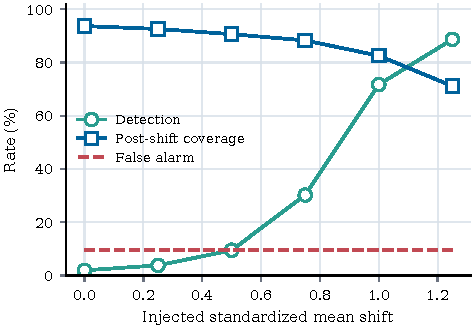
\includegraphics[width=\columnwidth]{figures/fig_drift_sensitivity.pdf}
\caption{Detection rate, post-shift coverage, and trace-level false-alarm rate versus the injected standardized mean shift.}
\label{fig:drift-sensitivity}
\end{figure}

\begin{figure}[t]
\centering
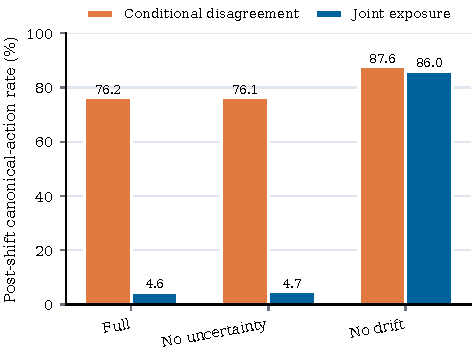
\includegraphics[width=\columnwidth]{figures/fig_drift_ablation.pdf}
\caption{Post-shift P4 conditional canonical-action disagreement and joint disagreement exposure for the full and ablated gates.}
\label{fig:drift-ablation}
\end{figure}

Figures~\ref{fig:drift-sensitivity} and \ref{fig:drift-ablation} show a low-power regime: at a .5-scale shift, detection is 9.43\% and post-shift coverage 90.64\%. Detection rises to 71.70\% at one scale and 88.68\% at 1.25 scales. The false-alarm line stays at 9.43\% because every sweep shares the same pre-change segment. Removing only functional uncertainty changes $E:76.23\%\to76.14\%$ and $J:4.57\%\to4.73\%$. Under severe shift, $I_t^\ell$ cannot substitute for timely epoch invalidation.

\subsection{Ablation and Sensitivity}

\begin{table}[t]
\caption{Mean stationary ablation results across P1--P3, with the mechanism retained by each variant.}
\label{tab:ablation}
\centering
\scriptsize
\setlength{\tabcolsep}{3pt}
\begin{tabular}{llrr}
\toprule
Variant & Retained mechanism & NRMSE & Agree (\%) \\
\midrule
No residual/temporal & contract normalization only & 0.854 & 87.78 \\
No temporal & current report only & 0.751 & 88.47 \\
Linear residual & ridge instead of trees & 0.713 & 88.81 \\
No typed contract & statistical fit; no type rejection & 0.695 & 89.32 \\
\textbf{Full} & contracts + temporal nonlinear residual & 0.694 & 89.34 \\
\bottomrule
\end{tabular}
\end{table}


Table~\ref{tab:ablation} gives the reconstruction sequence $.854\to.751\to.713\to.694$ for contract-only, anchor ridge, temporal ridge, and the full nonlinear map. Removing typing gives .695 because the benchmark preserves column order and paired anchors. This negative result is informative: typing is justified by the invariant $T_{ik}=0\Rightarrow(i,k)\notin E_v$, not by manufacturing an accuracy gain on already paired columns. The executable compiler accepts declared conversions/permutations and rejects quantity and scope decoys (4/4 checks); the untyped variant cannot. The benchmark materializes 369,492 certificates, totaling $369{,}492\times48=17{,}735{,}616$ bytes.

\begin{figure}[t]
\centering
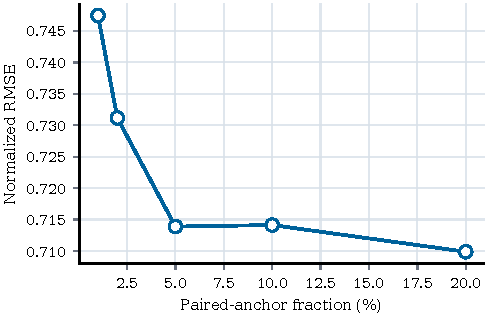
\includegraphics[width=\columnwidth]{figures/fig_anchor_sensitivity.pdf}
\caption{P3 reconstruction error versus the paired-anchor fraction. The curve shows diminishing returns beyond the initial anchor increase.}
\label{fig:anchor-sensitivity}
\end{figure}

\begin{figure}[t]
\centering
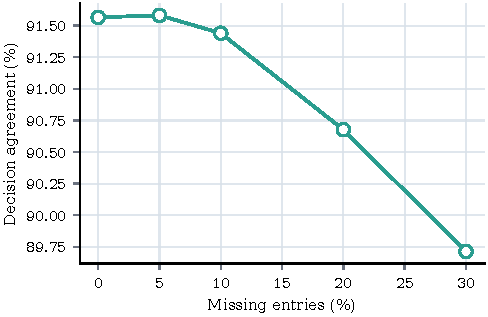
\includegraphics[width=\columnwidth]{figures/fig_missingness_sensitivity.pdf}
\caption{Fixed-xApp decision agreement when a P1 mapper trained at 3\% loss is evaluated under increasing missing-entry rates without refitting.}
\label{fig:missingness-sensitivity}
\end{figure}

\begin{figure}[t]
\centering
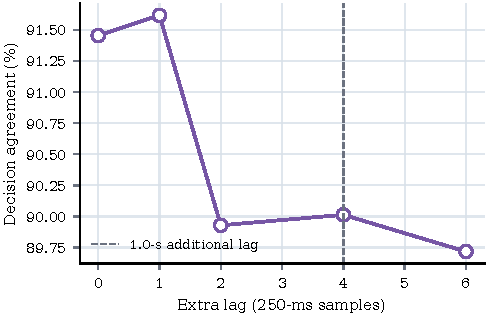
\includegraphics[width=\columnwidth]{figures/fig_lag_sensitivity.pdf}
\caption{Fixed-xApp decision agreement under unseen additional lag. The dashed line marks the one-second age increment reached at four 250-ms samples.}
\label{fig:lag-sensitivity}
\end{figure}

Figures~\ref{fig:anchor-sensitivity}--\ref{fig:lag-sensitivity} isolate anchor fraction $\eta_A$, unseen loss $p_m$, and extra lag $\Delta L$. For P3, $\eta_A:1\%\to5\%$ lowers NRMSE $.760\to.724$, while 20\% yields .721, showing diminishing returns in \eqref{eq:training-objective}. A P1 mapper fitted at $p_m=.03$ is tested without refitting: agreement decreases $90.15\%\to88.34\%$ as $p_m:0\to.30$ and the mask/support components of $x_t$ deteriorate. Expected one-sample lag gives 90.13\%; removing it gives 89.21\%, and $\Delta L\ge2$ lowers agreement below 87.6\%. Six samples also violate the 1.5-s age budget, so $G_t=0$ even if $M_v$ returns a vector.

\section{Complexity, Overhead, and Deployment}
\begin{figure}[t]
\centering
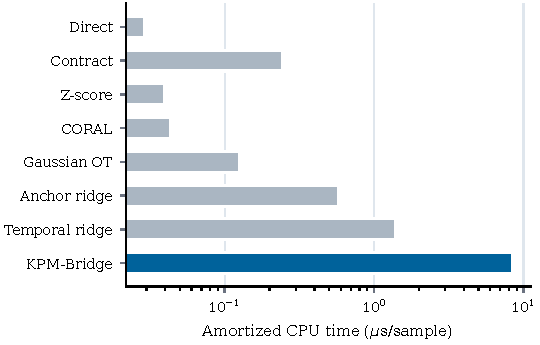
\includegraphics[width=\columnwidth]{figures/fig_runtime.pdf}
\caption{Amortized single-thread processor inference time per sample for KPM-Bridge and all portable baselines; the horizontal axis is logarithmic.}
\label{fig:runtime}
\end{figure}

The Python reference runs on an AMD EPYC 9V74 central processing unit (CPU) with one OpenMP/BLAS thread. A profile fit takes \BridgeFitRange; amortized inference is \BridgeLatency\ per sample and mean storage \BridgeModelSize. Temporal ridge takes \TemporalLatency\ and 13.4~KiB. Figure~\ref{fig:runtime} and Table~\ref{tab:complexity} separate observed $(T_{\rm fit},T_{\rm inf},M)$ from asymptotic scaling. E2 decoding, transport, scheduling, queueing, and actuation are excluded, so these are not worst-case deadlines.

\begin{table*}[t]
\caption{Asymptotic computation, persistent state, and measured reference cost by KPM-Bridge lifecycle stage.}
\label{tab:complexity}
\centering
\scriptsize
\setlength{\tabcolsep}{5pt}
\begin{tabular}{lllll}
\toprule
Stage & Trigger & Time complexity & Persistent memory & Reference observation \\
\midrule
Contract assignment & schema/policy change & $O((p_v+d)^3)$ & $O(p_vd)$ costs & negligible for eight targets \\
Counter/event-time update & every report & $O(hd)$ & $O(hd)$ history & included in mapper timing \\
Gradient-boosted mapping & every report & $O(dN_{\rm tr}L_{\rm tr})$ & $O(dN_{\rm tr}N_{\rm leaf})$ & \BridgeLatencyRange\ batched \\
Generic/functional gate & every report & $O(d)$ & $O(1)$ quantiles & fixed 48-byte certificate \\
Mean-shift monitor & trusted anchor & $O(d^2+Wd)$ & $O(d^2+Wd)$ & once per 2.5~s in benchmark \\
Refit/recalibration & invalid epoch & offline/model dependent & calibration buffer & \BridgeFitRange\ profile fit \\
\bottomrule
\end{tabular}
\end{table*}

The source cadence is $T_s=250$~ms and the QoS horizon is $4T_s=1$~s. Although measured batch compute is small relative to $T_s$, deployment requires a tail budget $T_{.99}^{\rm dec}+T_{.99}^{\rm trans}+T_{.99}^{\rm sched}+T_{.99}^{\rm cert}+T_{.99}^{\rm inf}+T_{.99}^{\rm act}\le B_t$.

At report rate $r$, $N$ UEs, and $V$ certified views, certificate throughput is $B_\gamma=48rNV$ bytes/s. For $(r,N,V)=(10,100,1)$, $8B_\gamma=$\HundredUeCertificateRate; adding an eight-float32 vector gives 0.640~Mbit/s before headers. The evaluated sidecar remains inside the Near-RT RIC and does not alter E2 subscriptions; external transport would add protocol and security headers.

Compilation runs only when the schema or policy version changes. Per implementation, streaming state contains nine report positions, masks, age/support, model state, and drift statistics. After compilation, work is $O(|\cV|)$ across E2 nodes and can be sharded. Production still requires a compact tree runtime and tail-latency measurements on the target RIC.

\section{Discussion and Limitations}
\emph{Certificate interpretation:}
The certificate binds $(C_v,\pi_v,M_v,e,\gamma_t)$ to measured operating evidence. Its finite-sample statement requires exchangeability and does not imply conditional coverage for every subgroup. Nor does $G_t=1$ prove that the xApp is beneficial, fair, secure, or stabilizing. The object certifies telemetry fitness under a declared regime, not system trustworthiness.

\emph{Information loss and anchors:}
If $\ker(A)\neq\{0\}$, cell aggregation cannot identify per-UE state without side information; long windows suppress transients and consecutive losses reduce support. The correct response is a larger $\cU_t$ or $G_t=0$, not invented detail. A cybersecurity-driven quantum digital twin likewise maps O-RAN observations into detection registers \cite{alkarawi2026cqdt}; KPM-Bridge can guard the compatibility of those inputs but cannot validate the twin's policy. The 10\% anchor budget requires a trusted reference, twin, temporary dual report, or validated probe. Results remain useful at 5\%, yet anchor cost and integrity are deployment constraints.

\emph{Controlled profiles versus vendors:}
P1--P4 are controlled transforms $\Psi_p$ over a public experimental corpus, not measurements of commercial products. Static UEs and $T_s=250$~ms limit generalization to mobility, handovers, multi-cell conversion, and faster loops. Vendor studies should disclose, where permitted, schemas, timestamp behavior, aggregation/reset tests, and anchor procedures.

\emph{Contract governance and versioning:}
Operator-governed contracts bind quantity/scope namespaces, E2SM revision, measurement identifier, labels, canonical ontology, and transform hash. A unit conversion may preserve $T_{ik}=1$; a UE-to-cell change makes $T_{ik}=0$; and a window or clock change invalidates epoch $e$. The operator, not the xApp, approves sources against model-card requirements for features, age, support, and $I_t^\ell$.

\emph{Calibration under time dependence:}
Split-conformal coverage is finite-sample exact for exchangeable calibration units. Experiment separation and subsampling reduce but do not remove dependence. The measured \StableCoverage\ at nominal $1-\alpha=95\%$ motivates block-aware or weighted calibration \cite{barber2023exchangeability}.

\emph{Drift and false alarms:}
Without trusted anchors, $H_t$ cannot observe drift. Under P4, detection is imperfect, \DriftFalseAlarm\ of traces alarm before the shift, and conditional post-shift disagreement remains \DriftSelectiveError. The main benefit is \DriftExposureReduction\ lower $J_{\rm exp}=A_{\rm acc}E_{\rm sel}$, achieved through abstention. Lowering $h_{.975}$ trades delay for availability, and the per-stream-maximum threshold is empirical rather than an anytime-valid false-alarm theorem. Alarms need cause codes and operator diagnostics. Corrupting both reports and anchors can evade residual monitoring, while induced missingness can force denial of service. Authenticated anchors, execution controls, rate limits, redundant evidence, and emergency policy remain platform responsibilities.

\emph{External validity:}
External validation should compose xDevSM with KPM-Bridge on OAI, srsRAN, and vendor E2 traces while varying $(w,\tau,\rho)$, mobility, and schedulers. Conditional or block-aware calibration, monotone maps, and cost-aware selection of $\mathcal D_v^A$ remain open.

\section{Reproducibility}
Source, pinned manifests, tests, and generated artifacts are available in the \href{https://github.com/YassirALKarawi/kpm-bridge-open6g-ran}{KPM-Bridge repository}. One command regenerates the evidence; upstream GPL-3.0 traces are not redistributed.

\section{Conclusion}
KPM-Bridge separates successful E2/API decoding from the stronger claim that $y_{v,t}$ is a valid input for a fixed xApp. Typed matching prevents quantity and scope substitution, the causal map repairs declared counter and temporal differences, $(\cU_t,I_t^\ell)$ expose uncertainty, and $H_t$ invalidates a stale epoch. On independent ColO-RAN repetitions, the observed stationary NRMSE is lower and canonical-decision agreement higher than for the evaluated portable baselines, with overlapping whole-trace intervals reported explicitly. Under severe drift, fail-closed gating reduces joint disagreement exposure $J_{\rm exp}$ by \DriftExposureReduction, but accepts only 5.99\% of post-shift samples; large conditional disagreement, delay, and false alarms remain. A portable xApp should therefore receive $(\hat z_t,\gamma_t)$, not an unqualified KPM vector.

\section*{Acknowledgment}
The authors used OpenAI ChatGPT for language editing and assistance with reproducibility code. They reviewed and verified the manuscript, equations, references, code, and reported results and remain responsible for the content.

\bibliographystyle{IEEEtran}
\IEEEtriggeratref{19}
\bibliography{references}
\end{document}
